\section{\textit{Motion capture-driven simulations that hit and react}}

% ============================================================================
\subsection{Referência completa do artigo}

\begin{itemize}
  \item \textbf{Autores:} Victor B. Zordan, Jessica K. Hodgins
  \item \textbf{Local:} College of Computing and GVU Center, Georgia Institute of Technology
  \item \textbf{\textit{Journal}:} SIGGRAPH Symposium on Computer Animation [Qualis A2]
  \item \textbf{Data:} 21-26 July 2002
  \item \textbf{Referência:} \citeonline{bib:2002:cms}
\end{itemize}

% ============================================================================
\subsection{Resumo}

\subsubsection{Abstract}

Controllable, reactive human motion is essential in many video games and training environments. Characters in these applications often perform tasks based on modified motion data, but response to unpredicted events is also important in order to maintain realism. We approach the problem of motion synthesis for interactive, human-like characters by combining dynamic simulation and human motion capture data. Our control systems use trajectory tracking to follow motion capture data and a balance controller to keep the character upright while modifying sequences from a small motion library to accomplish specified tasks, such as throwing punches or swinging a racket. the system reacts to forces computed from a physical collision model by changing stiffness and damping terms. The free-standing, simulated humans respond automatically to impacts and smoothly return to tracking. We compare the resulting motion with video and recorded human data.

% ..........................................................
\subsubsection{Motivação}
Para conseguir movimentos realistas, é interessante estudar a técnica de captura de movimentos e como os dados de captura podem ser modificados para adequar a animação a cada situação, como reação a um obstáculo móvel.

% ..........................................................
\subsubsection{Propósito do artigo}

A ideia do artigo é partir de um banco de movimentos previamente capturados, que possuem características naturais e trazem menos estranhamento ao serem vistos, e tentar obter uma animação final, fisicamente realista, com transições suaves entre as poses de forma que seja gerada uma animação desejada.

% ..........................................................
\subsubsection{Técnicas utilizadas} 
\begin{itemize}
  \item Motion Capture
  \item Controladores
  \item Cinemática Inversa
  \item Blending de animações
\end{itemize}  

% ..........................................................
\subsubsection{Contribuição em relação a artigos anteriores} %mais ou menos 10 linhas
 \begin{itemize}
   \item x
 \end{itemize}  

% ============================================================================
\subsection{Metodologia}
% Descreva um pouco mais detalhadamente a metodologia e os resultados do artigo. 
% Inclua as figuras que achar mais relevantes.

\subsubsection{Introdução}

O objetivo é combinar dois objetivos, muitas vezes conflitantes: permanecer proximo o suficiente do dado capturado original, para manter características importantes da animação real e desviar o suficiente deste resultado para atingir outro objetivo, dada uma tarefa.

\subsubsection{Editando motion capture}

Diversas tecnicas existem para essa tarefa. Interpolação de keyframes, adaptando o movimento para um novo personagem mantendo os contatos e alterando a dinâmica da animação, usando b-splines. Para a implementação sugerida pelo artigo, eles realizam pequenas edições na animação original, e essa animação modificada será o input para a simulação que é feita em seguida.
Outro problema existente é como combinar mais de uma animação. Uma possibilidade seria decompor dois movimentos bem diferentes em bandas de frequencia e permitir o usuário controlar o blending entre essas frequencias. Outra possibilidade é utilizar uma expansão da série de fourrier para interpolar entre sequencias de movimentos parecidos, como corrida, pulo e andar. Outras tecnicas tentam mapear posições chaves para fazer transições suaves de uma animação para outra, como andar triste e andar alegre, que possuem uma pose em comum. Todas as tecnicas mencionadas podem ser utilizadas, dependendo da situação.

\subsubsection{Humanos baseados em física}
Personagens humanoides completamente simulados oferecem potencial para uma animação mais complexa e realista, interagindo com outros personagens e objetos da cena. Alguns trabalhos anteriores partiam de movimentos estimados, e passavam por um processo de otimização até encontrar uma animação melhor, segundo algum critério estabelecido, e que respeita as restrições do ambiente. Adicionado as forças internas, um sistema de balanço que aplica forças externas poderia ser adicionado para simplificar o processo. Para a implementação do artigo, ele combina movimentos primitivos e maquinas de estado de alto nível para compor os movimentos finais da animação.

\begin{figure}[ht]
  \centering
  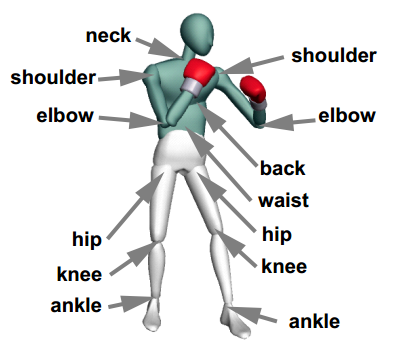
\includegraphics[height=150px]{artigos/2002_SCA_Motion_capture-driven_simulations_that_hit_and_react_p89-zordan/fig_model.png}
  \caption{Cada uma das juntas possui três graus de liberdade. Os valores de massa e parâmetros de inércia são calculados baseados nos modelos geométricos e nas medidas de densidade humana.}
  \label{fig:2002:mocap_sim:fig1}
\end{figure}

\subsubsection{Controle baseado em motion capture}

Os modelos utilizados, como dito anteriormente, são figuras humanas. Na figura \ref{fig:2002:mocap_sim:fig1} vemos os graus de liberdade do modelo humano utilizado para os experimentos. O nó raiz do movimento é considerado na pelvis. 
Para conseguir o controle dos movimentos capturados, um controlador de trajetória e um algoritmo que combina sequencias de movimentos capturados. O Torque de cada junta é calculado por um controlador "proporcional-derivado".

\begin{equation}
  \label{eq:2002:mocap:pdcontroller}
	\tau_t = k_t (\theta_d - \theta) - b_t (\dot{\theta})
\end{equation}

Assim como no artigo anterior. Agora é possivel o personagem seguir os dados de captura. 
Para tornar mais preciso, o sistema pode considerar o momento de inercia de toda a cadeia afetada pela junta, fazendo com que o número de parâmetros para ajustar as juntas do corpo sejam reduzidas, podendo ser até mesmo a mesma para todo o modelo, aumentando a velocidade e melhorando o desempenho do processo de ajuste.
Vale lembrar que sem o devido controle de feedback ou de interação com o ambiente, o personagem provavelmente iria cair sem fazer nada.

\subsubsection{Controle para bater}
Para criar animações que precisam de maior precisão e agilidade, como um soco, a técnica pura não pode ser utilizada. Para o exemplo do soco, foi feito um controle sobre o efetor final das mãos de forma que a animação atinja a posição desejada, e ajustando a escala de tempo para que a duração seja apropriada.
Primeiramente é utilizada uma solução de cinemática inversa para ajustar a posição do movimento bruto da captura. Isso permite novos movimentos que não estavam na biblioteca serem executados também.
Uma máquina de estados é adicionada para ter maior controle sobre a animação, como podemos ver na figura \ref{fig:2002:mocap_sim:fig2}.

\begin{figure}[ht]
  \centering
  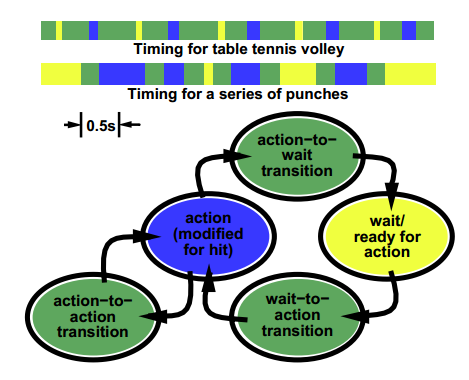
\includegraphics[height=150px]{artigos/2002_SCA_Motion_capture-driven_simulations_that_hit_and_react_p89-zordan/fig_state.png}
  \caption{Máquina de estados para o soco e para a cena da raquete. A cor das barras indica a duração de cada estado para cada uma das animações.}
  \label{fig:2002:mocap_sim:fig2}
\end{figure}

O final de um segmento de animação é interpolado com o segmento seguinte. Ações são enfileiradas para quando uma atividade chegar ao fim, a próxima iniciar.

\subsubsection{Reagindo a contatos}

O valor de ajuste, se muito alto, pode fazer com que a animação fique muito proxima da captura de movimento, e ignorando a simulação de impacto. Uma possibilidade é mudar o valor do ajuste de acordo com a ação que está acontecendo. Apenas os valores da região do corpo afetadas pelo movimento podem ser ajustadas, para dar o maior realismo possível para a animação.

\subsubsection{Equilibrando e rastreando}

A ideia do equilíbrio está relacionada ao centro de massa. Muitas ideias de controladores de equilibrio tentam minimizar a velocidade ou a aceleração do centro. A diferença dos problemas comuns para este é que a parte de baixo do corpo também está sob controle da captura de movimento.
Para conseguir o equilibrio, duas técnicas foram combinadas. Um "atuador virtual" calcula forças virtuais, e transforma elas em torques nas juntas, que representam o que o personagem pode fazer para se equilibrar com sua propria musculatura. Esse torque calculado é combinado com o torque da captura de movimento.
O intuito é manter o centro de massa proximo o suficiente de um centro de suporte, ponto simples de ser calculado baseado no polígono de apoio do personagem.

% ..........................................................
\subsubsection{Resultados}

Foram implementados diversos exemplos para ilustrar diversos aspectos do sistema.
No exemplo do tênis de mesa, o desafio era atingir uma bola em movimento a fim de mandá-la com uma determinada direção e velocidade. Portanto, a posição, orientação e velocidade da raquete precisam ser controladas.
No exemplo do boxe, considerado a maior contribuição do trabalho, foi a criação de um personagem a partir de dados de captura que podem interagir de maneira genérica. Animações de diferentes tipos de soco são modificadas utilizando cinemática inversa, fazendo com que o pugilista atinja posições epecíficas. Além disso, um personagem atinge o outro, sendo possível testar também a simulação de impacto, o equilíbrio e quanto o personagem consegue se manter proximo a sua simulação original.
No exemplo do personagem dançante, uma luva controlada pelo usuário pode interromper a animação com socos. Se a força for grande demais, o personagem pode até dar um passo involuntário para manter o equilíbrio. 

\begin{figure}[ht]
  \centering
  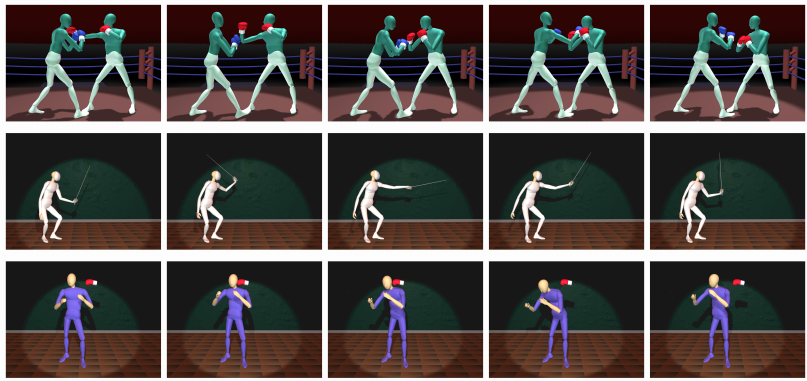
\includegraphics[height=150px]{artigos/2002_SCA_Motion_capture-driven_simulations_that_hit_and_react_p89-zordan/fig_examples.png}
  \caption{Exemplos para testar casos específicos de animação. Boxe, esgrima e um personagem dançando sendo atingido na cabeça.}
  \label{fig:2002:mocap_sim:fig3}
\end{figure}

% ============================================================================
\subsection{Pontos fortes} %no máximo três
\begin{itemize}
  \item Simulação combina mocap com restrições físicas para o corpo do personagem inteiro.
  \item Permite flexibilidade ao combinar com outras tecnicas de animação para permitir modificação dos dados brutos de captura.
\end{itemize}  

% ============================================================================
\subsection{Limitações} %no máximo três
\begin{itemize}
  \item A simulação em cima da captura de movimentos pode tornar a animação "suave", dificultando certas ações de acontecerem.
  \item A ideia de deixar mais automatico possivel se perde quando é preciso criar um grafo de controle de poses especiais.
\end{itemize} 


% ============================================================================
\subsection{Avaliação}
%\textbf{(a) Avanço considerável (\textit{Breakthrough}).}
 \textbf{(b) Contribuição significativa.}
% \textbf{(c) Contribuição modesta.}
% \textbf{(d) Contribuição fraca.}
% \textbf{(e) Sem contribuição.}
Muitos artigos semelhantes já existem na área. Porém é uma contribuição considerável visto o ganho de desempenho e o controle das ações mais detalhadas, através da máquina de estados.
Mas a parte mais significativa do artigo é a reação a impactos. A simulação resiste a diversos tipos de interações com os personagens, tentando manter a animação original na medida do possível, mas sem perder o realismo.

% ============================================================================
\subsection{Problema em aberto}
 \begin{itemize}
   \item Combinar simulação e animação de forma realmente automática. Muitos tipos de animação não podem ser obtidos a partir do dado bruto capturado, sendo necessária a interferência de um animador.
   \item O cálculo do impacto pode requerer mais precisão a medida que mais detalhes forem sendo adicionados à animação. O sistema atual funciona sob diversas restrições, como remoção de partes do corpo com pouca massa ou juntas desnecessárias para a animação a nível macroscópico.
 \end{itemize}  

% ============================================================================
\subsection{Aspecto obscuro}
 \begin{itemize}
   \item Não parece haver uma técnica para decidir quais aspectos implementar para cada animação. Parece que cada animação diferente requer uma adição à tecnica original para funcionar.
 \end{itemize}  